\documentclass[a4 paper]{article}
% Set target color model to RGB



\usepackage[inner=2.0cm,outer=2.0cm,top=2.5cm,bottom=2.5cm]{geometry}
\usepackage{setspace}
\usepackage[rgb]{xcolor}
\usepackage{verbatim}
\usepackage{subcaption}
\usepackage{amsgen,amsmath,amstext,amsbsy,amsopn,tikz,amssymb,tkz-linknodes}
\usepackage{fancyhdr}
\usepackage[colorlinks=true, urlcolor=blue,  linkcolor=blue, citecolor=blue]{hyperref}
\usepackage[colorinlistoftodos]{todonotes}
\usepackage{rotating}
%\usetikzlibrary{through,backgrounds}

\usepackage{lmodern}
\usepackage[T1]{fontenc}
\usepackage[capposition=top]{floatrow}
\usepackage{hyperref}
\usepackage{graphicx}
\graphicspath{ {images/} }
\usepackage{booktabs}
\usepackage{changepage}
\usepackage{float}








\hypersetup{%
pdfauthor={Nick Korbit},%
pdftitle={Homework},%
%pdfkeywords={Tikz,latex,bootstrap,uncertaintes},%
pdfcreator={PDFLaTeX},%
pdfproducer={PDFLaTeX},%
}
%\usetikzlibrary{shadows}
% \usepackage[francais]{babel}
\usepackage{booktabs}


\newcommand{\ra}[1]{\renewcommand{\arraystretch}{#1}}

\newtheorem{thm}{Theorem}[section]
\newtheorem{prop}[thm]{Proposition}
\newtheorem{lem}[thm]{Lemma}
\newtheorem{cor}[thm]{Corollary}
\newtheorem{defn}[thm]{Definition}
\newtheorem{rem}[thm]{Remark}
\numberwithin{equation}{section}

\newcommand{\homework}[6]{
   \pagestyle{myheadings}
   \thispagestyle{plain}
   \newpage
   \setcounter{page}{1}
   \noindent
   \begin{center}
   \framebox{
      \vbox{\vspace{2mm}
    \hbox to 6.28in { {\bf ISYE 6420:~Bayesian Statistics \hfill {\small #2}} }
       \vspace{6mm}
       \hbox to 6.28in { {\Large \hfill #1  \hfill} }
       \vspace{6mm}
       \hbox to 6.28in { {\it Instructor: {\rm #3} \hfill Name: {\rm #5}, gtID: {\rm #6}} }
       %\hbox to 6.28in { {\it TA: #4  \hfill #6}}
      \vspace{2mm}}
   }
   \end{center}
   \markboth{#5 -- #1}{#5 -- #1}
   \vspace*{4mm}
}

\newcommand{\problem}[2]{~\\\fbox{\textbf{Problem #1}}\newline\newline}
\newcommand{\subproblem}[1]{~\newline\textbf{(#1)}}
\newcommand{\D}{\mathcal{D}}
\newcommand{\Hy}{\mathcal{H}}
\newcommand{\VS}{\textrm{VS}}
\newcommand{\solution}{~\newline\textbf{\textit{(Solution)}} }

\newcommand{\bbF}{\mathbb{F}}
\newcommand{\bbX}{\mathbb{X}}
\newcommand{\bI}{\mathbf{I}}
\newcommand{\bX}{\mathbf{X}}
\newcommand{\bY}{\mathbf{Y}}
\newcommand{\bepsilon}{\boldsymbol{\epsilon}}
\newcommand{\balpha}{\boldsymbol{\alpha}}
\newcommand{\bbeta}{\boldsymbol{\beta}}
\newcommand{\0}{\mathbf{0}}



%%%%%%%%%%%%%%%%%%%%%%%%%%%%%%%%%%%%%%%%
%%			 Document				  %%
%%%%%%%%%%%%%%%%%%%%%%%%%%%%%%%%%%%%%%%%


\begin{document}
	
\homework{Homework \#4}{Spring 2020}{Roshan Vengazhiyil, Brani Vidakovic}{}{Nick Korbit}{903263968}


%%%%%%%%%%%%%%%%%%%%%%%%%%%%%%%%%%%%%%%%
%%			 Problem 1				  %%
%%%%%%%%%%%%%%%%%%%%%%%%%%%%%%%%%%%%%%%%




\problem{1}

\textbf{a$)$.} If we observe $n$ i.i.d. data points
distributed as $(X, Y) \sim \mathcal{M} \mathcal{V} \mathcal{N}_{2}(\mathbf{0}, \Sigma)$,
we get the following likelihood:

\begin{align*}
h(\rho|x,y)	=\prod_{i=1}^{n}\left(\frac{1}{2\pi\sqrt{1-\rho^{2}}}\exp\left\{ -\frac{1}{2\left(1-\rho^{2}\right)}\left(x_{i}^{2}-2\rho x_{i}y_{i}+y_{i}^{2}\right)\right\} \right)=\\
=	\left(\frac{1}{2\pi\sqrt{1-\rho^{2}}}\right)^{n}\exp\left\{ -\frac{1}{2\left(1-\rho^{2}\right)}\sum_{i=1}^{n}\left(x_{i}^{2}-2\rho x_{i}y_{i}+y_{i}^{2}\right)\right\} 
\end{align*}

Applying log transform to the likelihood we obtain:

$$
log h(\rho|x,y)=-nlog\left(2\pi\sqrt{1-\rho^{2}}\right)-\frac{1}{2\left(1-\rho^{2}\right)}\sum_{i=1}^{n}\left(x_{i}^{2}-2\rho x_{i}y_{i}+y_{i}^{2}\right)
$$

We can write un-normalized posterior as:

$$
\pi(\rho|x,y)\propto\prod_{i=1}^{n}\left(\frac{1}{2\pi\sqrt{1-\rho^{2}}}\exp\left\{ -\frac{1}{2\left(1-\rho^{2}\right)}\left(x_{i}^{2}-2\rho x_{i}y_{i}+y_{i}^{2}\right)\right\} \frac{1}{\left(1-\rho^{2}\right)^{3/2}}\right)
$$

$$
\pi(\rho|x,y)\propto\prod_{i=1}^{n}\left(\frac{1}{2\pi\left(1-\rho^{2}\right)^{2}}\exp\left\{ -\frac{1}{2\left(1-\rho^{2}\right)}\left(x_{i}^{2}-2\rho x_{i}y_{i}+y_{i}^{2}\right)\right\} \right)
$$

$$
\pi(\rho|x,y)\propto\left(\frac{1}{2\pi\left(1-\rho^{2}\right)^{2}}\right)^{n}\exp\left\{ -\frac{1}{2\left(1-\rho^{2}\right)}\sum\left(x_{i}^{2}-2\rho x_{i}y_{i}+y_{i}^{2}\right)\right\} 
$$


Applying log transform to the posterior we obtain:

$$
log(\pi|x,y)\propto-nlog\left(2\pi\left(1-\rho^{2}\right)^{2}\right)-\frac{1}{2\left(1-\rho^{2}\right)}\sum_{i=1}^{n}\left(x_{i}^{2}-2\rho x_{i}y_{i}+y_{i}^{2}\right)
$$

$$
log(\pi|x,y)\propto-nlog2\pi-2nlog\left(1-\rho^{2}\right)-\frac{1}{2\left(1-\rho^{2}\right)}\sum_{i=1}^{n}\left(x_{i}^{2}-2\rho x_{i}y_{i}+y_{i}^{2}\right)
$$


\textbf{b$)$.} Before devising steps for the 
Metropolis-Hastings 
procedure we make two observations.

First, our proposal distribution is uniform
$\mathcal{U}\left(\rho_{i-1}-0.1, \rho_{i-1}+0.1\right)$.
We can calculate the density $f(x)$ of the uniform 
distribution as $f(x)=\frac{1}{b-a}$ or
in our case:

$$
f(x)=\frac{1}{\rho_{i-1}+0.1-\left(\rho_{i-1}-0.1\right)}=\frac{1}{0.2}=5
$$

So that our proposal distribution does not dependent on
$\rho$.


Second, knowing the statistics after 100 observations,
we can simplify $log(\pi|x,y)$ as

$$
\sum_{i=1}^{n}\left(x_{i}^{2}-2\rho x_{i}y_{i}+y_{i}^{2}\right)=\sum_{i=1}^{n}x_{i}^{2}-2\rho\sum_{i=1}^{n}x_{i}y_{i}+\sum_{i=1}^{n}y_{i}^{2}=220.8903-165.0494\rho
$$

$$
\pi(\rho|x,y)\propto\left(\frac{1}{2\pi\left(1-\rho^{2}\right)^{2}}\right)^{100}\exp\left\{ -\frac{220.8903-165.0494\rho}{2\left(1-\rho^{2}\right)}\right\} 	
$$





We now specify the Metropolis-Hastings 
procedure:

\begin{enumerate}
	\item Start with arbitrary $\rho_0$
	
	\item Generate proposal $\rho'$ from $\mathcal{U}\left(\rho_{i-1}-0.1, \rho_{i-1}+0.1\right)$
	
	\item Calculate acceptance probability 
	$\alpha$:

$$
\alpha\left(\rho_{n},\rho'\right)=\min\left\{ 1,\frac{\pi\left(\rho^{\prime}\right)}{\pi\left(\rho_{n}\right)}\frac{q\left(\rho_{n}|\rho'\right)}{q\left(\rho'|\rho_{n}\right)}\right\} 
$$

Taking into account our observations we can simply $\alpha$:
$$
\alpha\left(\rho_{n},\rho'\right)=\min\left\{ 1,\frac{\pi\left(\rho^{\prime}\right)}{\pi\left(\rho_{n}\right)}\right\} 
$$
where 
$$
\pi\left(\rho\right)=\left(\frac{1}{\left(1-\rho^{2}\right)^{2}}\right)^{100}\exp\left\{ -\frac{220.8903-165.0494\rho}{2\left(1-\rho^{2}\right)}\right\} 
$$


	\item Determine $\rho_{n+1}$ as
	\begin{itemize}
		\item $\rho_{n+1}=\rho'$ with probability $\alpha$
		\item $\rho_{n+1}=\rho_{n}$ with probability $1-\alpha$
	\end{itemize}
	
	
	\item Set $n =n+1$ and go to Step 2.
	
\end{enumerate}

\textbf{c$)$.} We now simulate 
51000 samples from the posterior. 
Burning the first 1000 samples
we plot the histogram of the last 50000 samples:

\begin{figure}[H]
	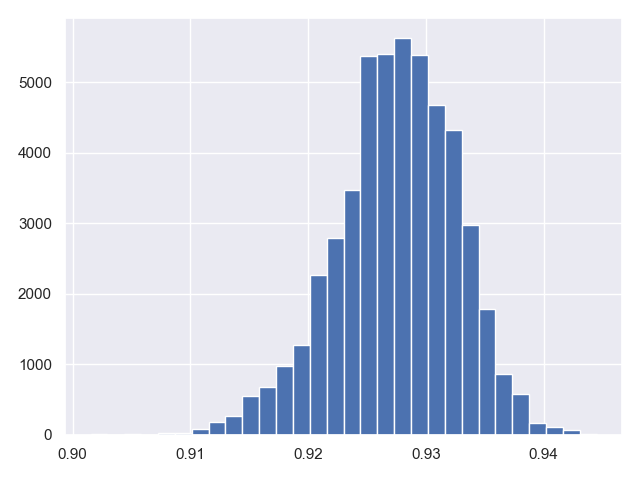
\includegraphics[scale=0.4]{q1a}
	\centering
	%	\caption{cdf .}
	\label{q1a}
\end{figure}

We see that the empirical distribution 
is unimodal, with a peak around $0.93$ value.
 
We also plot the last 1000 observations.

\begin{figure}[H]
	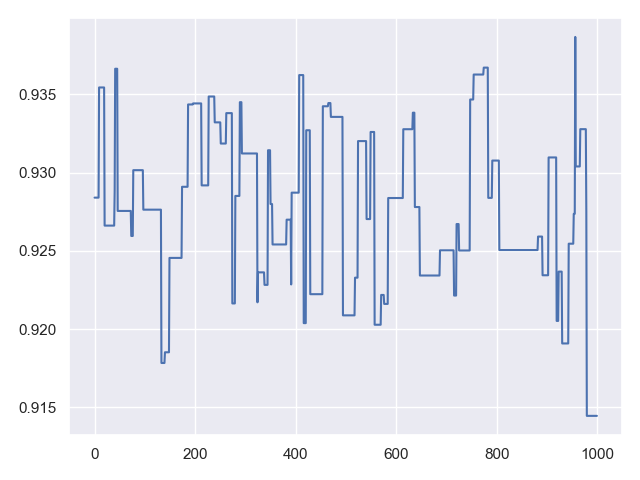
\includegraphics[scale=0.4]{q1b}
	\centering
	%	\caption{cdf .}
	\label{q1b}
\end{figure}


We notice that the majority of samples
are -1 with a small spike with values $(-1,-0.6)$.

Let's calculate Bayes' estimators: the mean 
of the simulated data is 0.9274
and the mode is 0.9307.


\textbf{d$)$.} Let's switch 
proposal distribution to the uniform 
$\mathcal{U}(-1,1)$. Plotting last 1000 samples will yield:

\begin{figure}[H]
	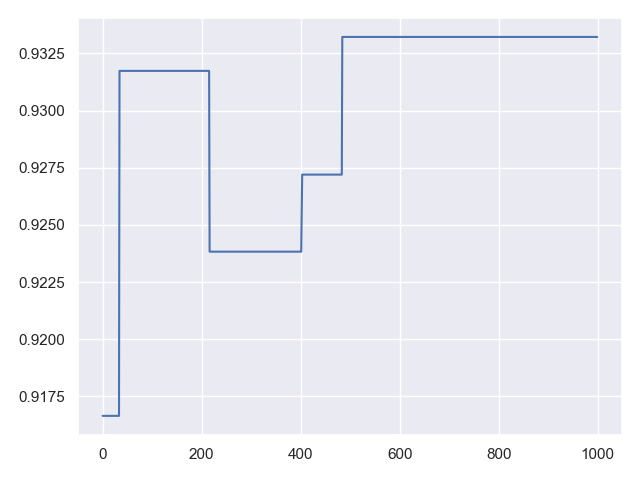
\includegraphics[scale=0.4]{q1c}
	\centering
	%	\caption{cdf .}
	\label{q1c}
\end{figure}

We see that using a pure sample from 
$\mathcal{U}(-1,1)$ will result in
discarding the majority of the samples 
in later stages of the simulation. Thus,
we might stick to the original distribution 
in order to generate 
samples that are accepted more often and
calculate more reliable statistics.




\problem{2}

\textbf{a$)$.} Let's start with a
joint distribution $f(T_{i},\lambda,\mu)$:


\begin{align*}
f(T_{i},\lambda,\mu)	=\left\{ \prod_{i=1}^{n}f\left(T_{i}|\lambda,\mu\right)\right\} \pi(\lambda)\pi(\mu)= 	\left\{ \prod_{i=1}^{n}\lambda\mu\exp\left\{ -\lambda\mu t_{i}\right\} \right\} \lambda^{c-1}\mu^{d-1}\exp\{-\alpha\lambda-\beta\mu\}= \\
=	\lambda^{n}\mu^{n}\lambda^{c-1}\mu^{d-1}\exp\{-\alpha\lambda-\beta\mu\}\exp\left\{ -\lambda\mu\sum_{i=1}^{n}t_{i}\right\} 
\end{align*}


We now find the full conditionals for
$\lambda$ and $\mu$ by selecting the terms 
from $f(T_{i},\lambda,\mu)$ that contain
$\lambda$ and $\mu$ respectively and
then normalize:
 
$$
f(\lambda|T_{i},\mu)	\propto\lambda^{n+c-1}\exp\left\{ -\lambda\left(\alpha+\mu\sum_{i=1}^{n}t_{i}\right)\right\} 
$$

We can recognize a $\mathcal{G}a(a, b)$ 
distribution of a general form $x^{a-1}e^{-b x}$
where in our case $a=n+c$ and 
$b=\alpha+\mu\sum_{i=1}^{n}t_{i}$. So that

$$
\left[\lambda | \mu, t_{1}, \ldots, t_{n}\right] \sim \mathcal{G} a\left(n+c, \mu \sum_{i=1}^{n} t_{i}+\alpha\right)
$$

Using the same derivation we can also state that 

$$
\left[\mu | \lambda, t_{1}, \ldots, t_{n}\right] \sim \mathcal{G} a\left(n+d, \lambda \sum_{i=1}^{n} t_{i}+\beta\right)
$$






\textbf{b$)$.} We now develop a Gibbs sampler 
procedure for our case. But first we
substitute $n$, $c$, $\alpha$, $\beta$, $\sum_{i=1}^{n} t_{i}$ 
with experimental data and hyperparameters. So that 
we can sample from:

$$
\left[\lambda|\mu,t_{1},\ldots,t_{n}\right]\sim\mathcal{G}a\left(23,512\mu+100\right)
$$

$$
\left[\mu|\lambda,t_{1},\ldots,t_{n}\right]\sim\mathcal{G}a\left(21,512\lambda+5\right)
$$

The algorithm is then:

\begin{enumerate}
	\item Start with $\mu_0=0.1$
	
	\item Sample initial $\lambda_0$ from $\mathcal{G}a(23,151.2)$ 

	\item Sample
	\begin{itemize}
		\item $\mu_{n+1}$ from $\left[\mu|\lambda,t_{1},\ldots,t_{n}\right]\sim\mathcal{G}a\left(21,512\lambda_n+5\right)$
		
		\item $\lambda_{n+1}$ from $\left[\lambda|\mu,t_{1},\ldots,t_{n}\right]\sim\mathcal{G}a\left(23,512\mu_{n+1}+100\right)$
	\end{itemize}
	
	
	\item Set $n =n+1$ and go to Step 3.
	
\end{enumerate}



\textbf{c$)$.} We now simulate 51000 paths
using the Gibbs sampler. We plot the 
histograms for $\lambda$ and $\mu$
and the scatter plot linking 
those variables:

\begin{figure}[H]
	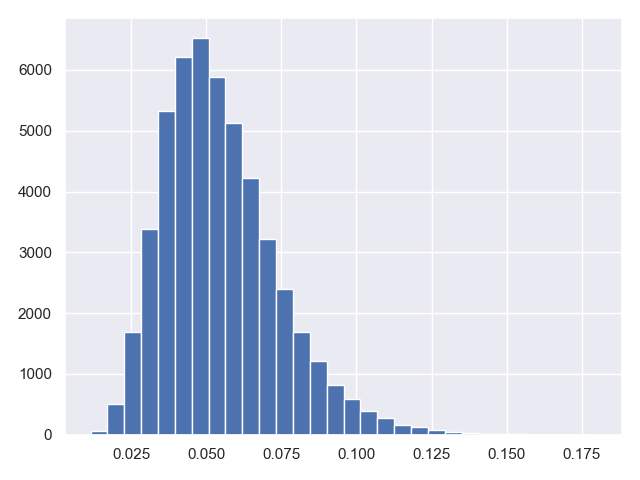
\includegraphics[scale=0.4]{q2a}
	\centering
	\caption{Distribution of Lambdas.}
	\label{q2a}
\end{figure}

\begin{figure}[H]
	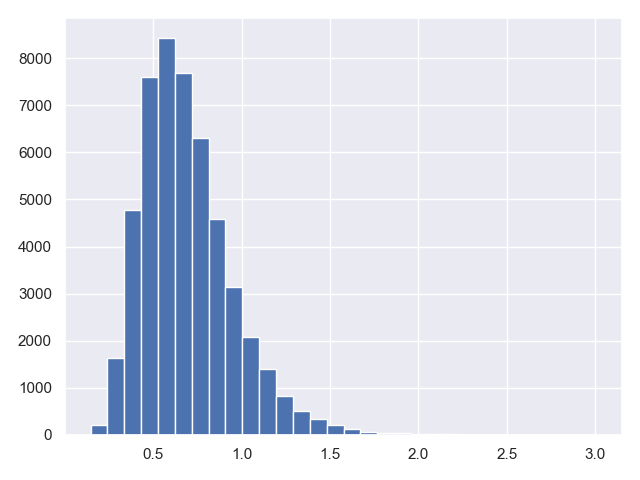
\includegraphics[scale=0.4]{q2b}
	\centering
	\caption{Distribution of Mus.}
	\label{q2b}
\end{figure}

\begin{figure}[H]
	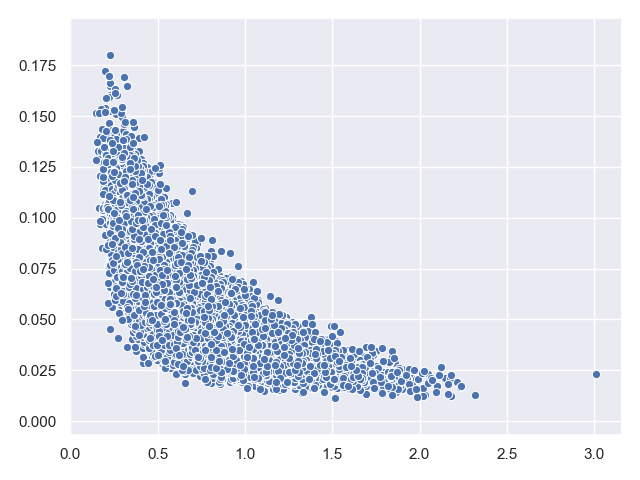
\includegraphics[scale=0.4]{q2c}
	\centering
	\caption{Scatter of Mus (x-axis) and Lambdas (y-axis).}
	\label{q2c}
\end{figure}

Let's calculate the statistics based on the simulated 
$\lambda$ and $\mu$:
\begin{itemize}
	\item $E\left[\lambda\right]\approx0.0548$
	\item $Var\left[\lambda\right]\approx0.0003667$
	\item 95-\% Equitailed credible set for $\lambda$ is [0.02569, 0.10013]
	\item $E\left[\mu\right]\approx0.69033$
	\item $Var\left[\mu\right]\approx0.06504$
	\item 95-\% Equitailed credible set for $\lambda$ is [0.3141, 1.30128]
\end{itemize}



\textbf{d$)$.} We can also calculate 
Bayes estimator by taking 
the average of the product of
$\lambda$ and $\mu$ $\approx$ 0.03426.



\textbf{Note}. The code for solving Q1 and Q2
is implemented in \textit{hw4.py}.
Just run \textit{python hw4.py}.


%%%%%%%%%%%%%%%%%%%%%%%%%%%%%%%%%%%%%%%%
%%			 Bibliography			  %%
%%%%%%%%%%%%%%%%%%%%%%%%%%%%%%%%%%%%%%%%

\begin{thebibliography}{9}


\bibitem{stat}\label{stat} 
Engineering Biostatistics: An Introduction using MATLAB and WinBUGS. 
Brani Vidakovic - Wiley Series in Probability and Statistics.

\end{thebibliography}



\end{document} 